\chapter{Ensemble Methods and  Naive Bayes Classifier}\label{ch:ensembleMethods}


\section{Classifier: Naive Bayes}

The Naive Bayes model encompasses a group of simple and computationally efficient algorithms which are built with a strong statistical assumption of independence among the features. Even though this belief is in practice wrong, the model still achieves acceptable classification rates for some problems. In addition, it does not suffer in problems of high-dimensionality, where $p >> n$ i.e.\ there are more attributes than samples in the data.

It is presented mostly for computational benchmark purposes, where in practice the classification rate achieved by this model serves as a baseline for other, more complex, learners. Furthermore, the algorithm has linear complexity in the number of features and samples $O(d+n)$, so it can be easily extended to \textit{larger} problem implementations. Furthermore, its maximum-likelihood estimation of the parameters has a closed form solution which is faster to compute over other iterative methods such as techniques using gradient descent or other similar iterative optimization routines.

Let $x = (x_1,\ldots,x_p)$ be any given data sample and $C_k$ be one of $K$ possible output classes of a classification problem. We take $p(C_k \mid x)$ to be the class posterior probability of this class given the sample.

In \cref{ch:machineLearning}
we have used
\begin{equation}
p(C_k| x) = \frac{P(x|C_k)P(C_k)}{P(x)}
\end{equation}\label{eq:equation-posteriorProbabilties}


and argued that if our data is given, then our model can only improve the posterior probability by optimizing $P(x|C_k)P(C_k)$ which is just the joint probability of the sample and the class.

Here we can approximate the posterior as

\begin{equation}
P(C_k \mid x) \approx p(C_k) * \prod_{j=1}^{p}  P(x_j \mid \bigcap_{k=j+1}^{p} x_k \cap C_k)
\end{equation}\label{eq:posteriorProbabilityDecomposition1}


We now impose a strong independence assumption among features, given the target class, to let the conditional probability factors become the probability of each feature. %This assumption is what gives the model its

This yields a posterior probability which depends only on the prior probability and on the individual likelihood of each feature.

\begin{equation}
P(C_k \mid x) \approx p(C_k) * \prod_{j=1}^{p}  P(x_j | C_k)
\end{equation}\label{eq:posteriorProbabilityDecomposition2}

As we have said before, the parameters of the model can only reweigh the likelihood factors, so if we look to maximize the posterior probability, our final estimate of the posterior will take the following form.

\begin{equation}
P(C_k \mid x) = \frac{1}{Z} p(C_k) * \prod_{j=1}^{p}  P(x_j | C_k)
\end{equation}\label{equation-posteriorProbabilityDecomposition3}

where in the equation $Z = p(x)$ is a scaling factor and is fixed to the dataset.

In practice, the model will stem into different algorithms where each variant will have a different probabilistic assumption on the likelihoods $p(x_j \mid C_k)$ of the model and on the priors $p(C_k)$. It is common to choose among using a nonparametric density estimations from the data or assuming that the data comes from an exponential family distribution such as a Gaussian, Bernoulli or Multinomial distributions. Different choices will certainly lead to different cross validation scores among problems. Altogether, these choices can be treated as part our model's hyperparameters and the best one can be selected with our CV procedure.
%Indeed,

Finally, the output class for a given sample will be given by taking the class $k'$ which maximizes the probability $P(C_k' \mid x)$.


\section{Classifier: Decision Trees}\label{section:decision_trees}

%view of this supervised learner used in regression and classification problems.

% The models builds a
Decision trees are such as in the graph theoretical sense where each node acts as a rule to which any input sample can comply or not. The rules are built as linear (or similar) partitions of input space and they are built on the value of a given feature
%properties of the values for each feature.

At any given node the model takes a decision to include or exclude a sample $s$ from that partition by checking if $X_i(s) \in U$ where $X_i$ might be any given feature of the data and $U$ is a subset of said feature's space.

For numerical features, the input space $X$ will be partitioned into $L$ and $R$ where $L$ of the form $(-\infty,c]$. The value $c \in \mathbb{R}$ is any given number predefined by the rule itself. In the same way, for categorical features $L$ will be a subset of the possible values of that feature.

Altogether, a tree defines a partition of feature space in disjoint regions $A_1,\ldots,A_K$ such that the tree's predicted output $\hat{y}$ for a sample $x$ is $c_k$ if the sample belongs to $A_k$. Here $c_k$ is one of the possible values taken by the target variable $y$ in the training set. And by the way trees were built, each $A_k$ is a hyper-rectangles in feature space.

\subsection{Decision Trees Formulation}\label{subsection:decision_trees_formulation}
In brief, the learner can be characterized by
\begin{equation}
h(X) = \sum_{k=1}^K c_k I(X \in A_k)
\end{equation}\label{eq:decisionTreeModel}

where $c_k$ is the value that our model estimates for samples in the $A_k$ region. Both of these will have to be learned by the model in the optimization procedure. %by minimizing its loss function

By the points given above, the algorithm needs to determine what is the best way to split a set of samples that flow through a decision node. The \textit{goodness of split} will be measured by the loss metric of the algorithm. Here, the criteria used to decide on node splits are called \textit{node impurity measures}.
%them according, in order to optimize a loss metric.

%at each node
Most variations for this machine learning model build rules in a greedy fashion, where node impurity measures are locally optimized at each node to decide on which is the best splitting value. The reason for doing this is because not doing so will result in an algorithm whose computational complexity is infeasible. Given that the construction of optimal binary decision trees is NP-Complete~\cite{decisionTreesNP}, the optimal rules for the tree are then fit sequentially.

In conclusion, at any splitting node we have to find the \textit{best} feature $X^p$ and value split $t$ for which to partition the data in
$A_L = \{x \in \mathcal{T} \ / \ x^p \leq t \} $ and $A_R = \{x \in \mathcal{T}\ / \ x^p> t \} $. Let $N_l$ and $N_r$ be $|A_L|$ and $|A_R|$ respectively. Then, to quantify the \textit{best} feature for this split the algorithm minimizes:

%\frac{1}{N_{left}}
%\frac{1}{N_{right}}

\begin{equation}
%\begin{split}
\min_{p,t} \big[ \min_{c_L }  \frac{1}{N_l}\sum_{x \in A_L(p,t) } L(y,c_L)    \ +  \min_{c_R}  \frac{1}{N_r}\sum_{x \in A_R(p,t) } L(y,c_R) \big]
%\end{split}
\end{equation}\label{eq:decisionTreeGreedyOptimization}

where $y$ is the target associated to our sample $x$ and $L(\cdot)$ is the loss function we have used to measure the quality of our split. Note that this can be done efficiently for a wide range of loss functions since the minimization can be done for each feature independently.

A tree is then grown in an iterative way from the top down\footnote{In this context the \textit{top} of a tree refers to the root of the tree.}, estimating the appropriate parameters at each rule split. All of the training set's samples would start at the top (the root node) and then travel down through the trees branches, in accordance to their fulfillment or not of each node's rule. A branch of the tree would stop growing once all samples at a node belong to the same target class.

Finally, we would have that the tree's leafs are the partition subsets over the input data and once a learner is fit, predicting targets for new samples is straightforward: the prediction of their target class will be the value given after traveling the sample down to its corresponding leaf node.

To illustrate this method, an instance is show in \cref{fg:rf-treeFigure}. This classification tree example is built for the two class problem of gender prediction using data from CDRs:
%[.{\textit{Woman}}]
\smallskip
\begin{figure}[h]\label{fg:rf-treeFigure}
\Tree[.{ $Calling\_Volume \leq 23$ } [.{$Province \in \{ San Luis, Chubut \} $} [.{$Time\_Weekend \geq 16$} [.{\textit{M}} ] [.{\textit{F}} ] ]
[.{$Calls\_Weekdays \leq 48$}
[.{ $Time\_Weekday \geq 17$} [.{\textit{M}} ] [.{\textit{F}} ]] [.{\textit{F}} ] ] ]
[.{$Calls\_Mondays \geq 2$} [.{$Province \in \{ Chubut, Cordoba \} $} [.{\textit{M}} ] [.{\textit{F}} ] ]
[.{\textit{M}} ]]]

\end{figure}

\smallskip


%[.{\textit{M}} ] [.{\textit{F}} ]

\subsection{Node Splitting Criteria \& Hyperparameters}\label{subsection:decision_trees_impurity_measures_hyperparameters}


The most used metrics to build each rule are the \textit{Gini impurity measure} and the \textit{entropy} or \textit{information gain} criterion. The former optimizes for misclassification error in the two resulting sets. Where it values the accuracy of the model if all samples were to be tagged with the most common target-label in that split. The latter optimizes for information entropy, which is analogous to minimizing \textit{Kullback-Leibler divergence} of the resulting sets with respect to the original set previous to the split.

In this model, the process of iteratively partitioning the samples in splits continues until a predefined tuning parameter limit will stop the optimization or when there is only a single target class for all samples at the node.

The hyper-parameters for this model include the length of the tree, the splitting rule threshold and the node impurity measures. From the descriptions previously given, we can list these directly:

\begin{itemize}
\item Max depth of the tree, or the number of allowed level of splits.
\item The criteria or measure used to select the best split feature at each node.
\item The leaf size or the total number of minimum samples allowed per leaf. Note that this is a limit imposed on branch depth.
\item Number of features selected to decide on the best split feature at each node.
\end{itemize}


Intuitively, it is natural to find that trees of longer depth will overfit the data since more complex interactions among variables will be captured by refining the partition on input space.
A trivial case would be to allow a tree to grow fully in depth to later assign to each sample in the training set its own self-contained region.
This would yield a model with virtually low bias yet with a very high prediction error.
As we've shown before, this situation produces and overfit model since it will fail to predict correctly on new samples.
Recall that this was described in \cref{figure:dtree_overfit_problem_2}.
Here the training scores and CV scores were compared on models with increasing tree depth which at some point started to overfit the training set by increasing the gap of the CV and training errors.

At the same time, having a tree which is too shallow will result in most cases in a biased algorithm.
This is because it results in an overly simple model incapable of correctly assigning labels.
We must then consider that the depth of a tree is a measure of the model's complexity and as such one of the most important hyperparameters of our model.

Another drawback of the decision tree model is the high variance instability.
Authors point out that two very similar datasets can grow two very different resulting trees.
This is due to the hierarchical nature of the splits, where errors randomly made in the first splits will be carried onward towards the leafs since samples continue down on a single branch.

For the reasons described, in this model it is important to control the depth of the trees built.
The most common method to do this grows a very large tree $T_0$ that will continue until it reaches a depth limit threshold that is very unrestrictive.
Then the tree will be pruned by removing branches and nodes to remove model complexity with only a slight loss of accuracy.

To expand on the idea of tree complexity control, let $T \subset T_0$ be a subtree of the first tree, where $T$ is obtained by pruning $T_0$. Here the partition regions $R_j$ will be associated to $T$'s terminal nodes or leafs, indexed by $j$, which $j \in \{1,\ldots,|T| \}$.

Given a loss function, and a problem with $K$ possible target classes, we can define the following values:
\begin{equation}
\begin{split}
N_j & = \mid \{x \in R_j \}\mid \\
\hat{p}_{jk} & = \frac{1}{N_j} \sum_{x \in R_j} I(y=k)\\
c_j & = argmax_{k} \ \hat{p}_{jk} \\
\end{split}
\end{equation}\label{eq:decisionTreePruneParameters}

As we have mentioned before, at each split we use the node impurity measure to quantify this action. Here, we will denote $Q_j(T)$ to be the impurity measure for region $j$. In addition, we list the three most used impurity measures of classification trees:

\begin{itemize}
\item Misclassification error: $ \displaystyle \frac{1}{N_j} \sum_{x \in R_j} I(y\neq c_j) = 1 - c_j $
\item Gini index: $ \displaystyle \sum_{k\neq k'} \hat{p}_{jk} \hat{p}_{jk'}  = \sum_{k=1}^{K} \hat{p}_{jk} (1 - \hat{p}_{jk}) $
\item Cross-entropy: $ \displaystyle \sum_{k=1}^{K} -\log(\hat{p}_{jk})\hat{p}_{jk} $
\end{itemize}


As an extension to the Gini index, it is also common to use a reweighed version of the sum.
A loss matrix is multiplied to the factors in each summand.
The matrix is reassigning weights to different cases of misclassification.
Indeed, these weights become practical when we have that a sample from class $k$ incorrectly assigned to class $k'$ might be less important than other misclassifications.

Let $L \in \mathbb R_{\ge 0}^{K \times K}$ where $L_{(k,k')}$ is the cost of misclassifying a class $k$ sample into $k'$.
Naturally we have that $L$ is a null diagonal matrix.
Then the Gini index's summands will take the reweighed form $L_{kk'} \hat{p}_{jk} \hat{p}_{jk'}$.

For the binary (two class) case $Q_j(T)$ can be expressed in simpler terms. If we consider $p$ to be the probability of success, then we have

\begin{itemize}
\item Misclassification binary error: $1 - \\max(p, 1-p)$
\item Gini binary index: $ 2p(1-p) $
\item Binary cross-entropy: $ -\log(p)p - \log(1- p)(1-p) $
\end{itemize}\label{decisionTreeCostFunctions}

In summary, we will have an impurity measure for each region $R_j$ and the algorithm will then aggregate all of them into a single measure called the \textit{cost complexity criterion}. The idea is that this loss function, as a function of a tree, will control the whole optimization procedure through the tree's parameters. The criterion will be managed to control the final model's bias and variance. We define it in the following way

\begin{equation}
C_\alpha(T) = \sum_{j=1}^{|T|} N_j Q_j(T) + \alpha|T|
\end{equation}\label{eq:decisionTreeCostComplexity}


Here $\alpha \in \mathbb{R}_{\geq 0}$ is a tuning parameter that values the trade-off between the tree complexity, as given by its depth, and the accuracy of the model as given by the measure we proposed in \cref{decisionTreeCostFunctions}. The idea is that given an $\alpha$ we find the subtree $T_{alpha} \subset T_0$ that minimizes \cref{eq:decisionTreeCostComplexity}.

There are various methods we could use to find the optimal subtree. As an example, here we give an example of the \textit{weakest link pruning} algorithm which goes as follows:
%must \textit{prune} the initially grown tree

Let $B(T) = \sum_{j} N_j Q_j(T) $ be our pure loss function, without any complexity cost added.~\cite{breiman-cart84} shows that we can find $T_{alpha}$ included in a sequence of trees built for this. This sequence is constructed by iteratively pruning the node $j$ that, when removed from the tree, creates the smallest increase in $B(T)$.


% \begin{landscape}%[ht!]
% %\begin{center}
% % \includegraphics[width=0.7\columnwidth]{}
% 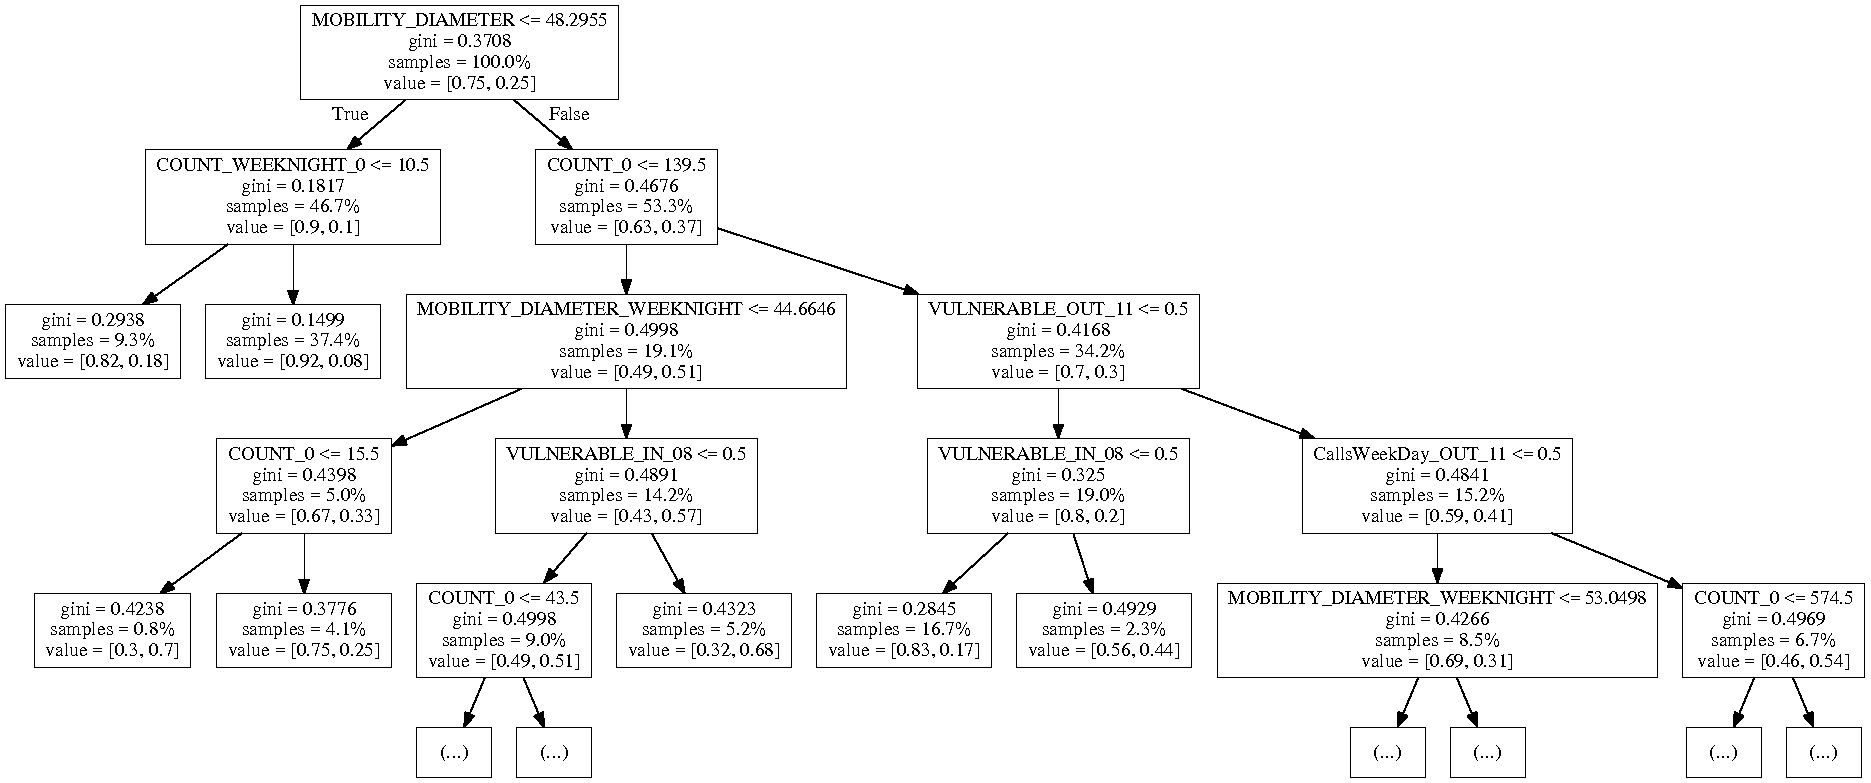
\includegraphics[width=\textwidth,height=\textheight,keepaspectratio]{figures/decision_tree/full_tree_map.png}
% \caption{ Example of a decision tree which has been pruned to fit the image. This was made on a CV procedure for \cref{target3}.}
% \label{fig:decision_tree_actual_problem}
% %\end{center}
% \end{landscape}


In this way, we'll have a sequence of trees $T_0,T_1,\ldots,T_l$ and a sequence of nodes $j_0, j_1,\ldots,j_l$ respectively the ones minimizing the increase in $B(T_0),B(T_1),\ldots,B(T_l)$ at each step. The algorithm will stop when have reached the root node and we will find our tree $T_{alpha}$ by comparing all the $C_\alpha(T)$ for all of the trees built in the sequence. In practice, it is common to have this procedure done within a $K$-fold cross validation routine to reach to an estimated $\hat{\alpha}$.

For a complete explanation of decision trees construction and uses in classification or regression problems, please refer to~\cite{breiman-cart84}.

\subsection{Experiment}\label{subsection:decision_trees_experiment}

We present here a run of the a decision tree over $\mathcal{T}$.
In this case the \cref{target2} was used as an example.
The tree was built using a standard configuration with a low depth of 5 and a Gini splitting criteria.
All features $X^j$ are available to be chosen at each split and a node has to have at least 20 samples to be split again. The algorithm ran in approximately 15 seconds.

\todo{fix decision tree horizontal, whole page, h! appearance}

\smallskip

\begin{figure*}[tb]
\centering
 \makebox[\textwidth]{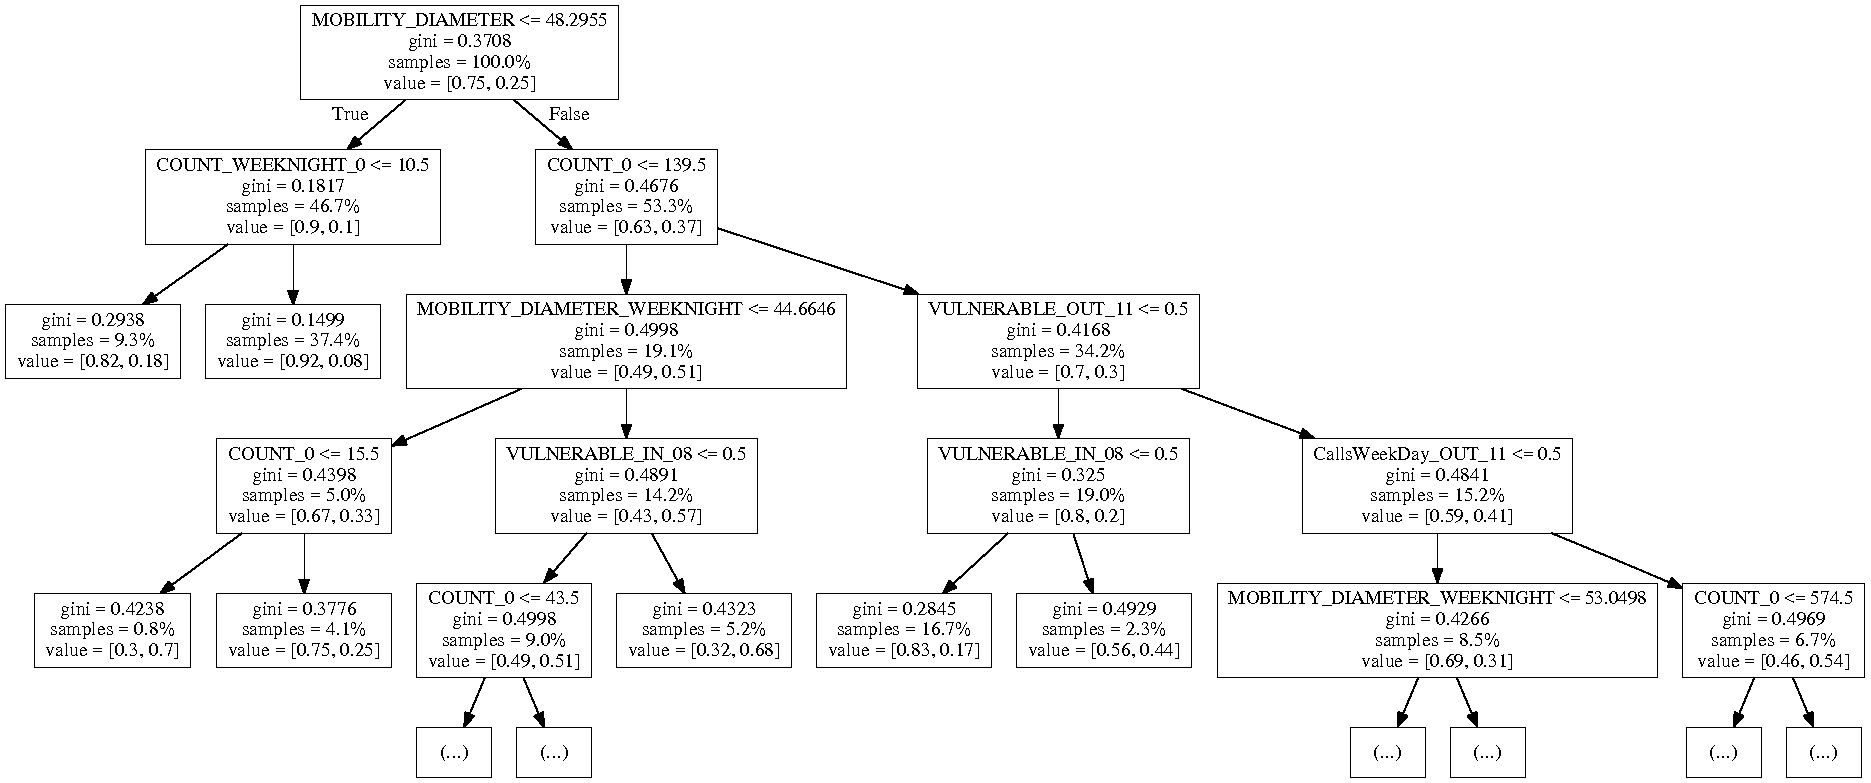
\includegraphics[width=.9\paperwidth]{figures/decision_tree/full_tree_map.png}}
\caption{ Example of a final decision tree. This model was made with a cross validated procedure on \cref{target3} and the resulting tree has been pruned to fit the image. For every node, the samples are split into sets given by the implicit indicator function defined in the condition.}
\label{fig:decision_tree_actual_problem}
\end{figure*}

\smallskip


From \cref{fig:decision_tree_actual_problem} we can approximate which features are most important to the algorithm when deciding a node split, given by the Gini splitting criteria.
Given that in \cref{target2} we are looking for people that migrated in any direction, the choice of the tree\'s root feature is not surprising.
The mobility diameter gives an idea of the area of influence of a user when using his mobile phone and as such, might be a proxy for migrations.
Subsequently, the volume of use of a user\'s home antenna appears as the second most important features, both during the weeknight and during the whole day.
Yet the error score out by this tree yields a poor performance. Evaluated with the $F1$ metric, we see 43.2\% result with this model which shows very poor prediction error over all of the samples.
With this, comparing how the top features result in the tree can be of little use to the overall problem.

We decide to iterate once again on this model, but now slightly changing the hyperparameter which controls the balance of $\mathcal{T}$.
The reason for this is that with the current task, the positive and negative classes have a disproportionate balance of samples and this is reflected in the overall model\'s poor performance.
For this reason, we modified the setup of the loss function of the tree to weigh more samples from the under-represented class over the samples from the abundant group.
For each sample, it\'s loss weight was adjusted by it\'s class representation ratio.
With this, the new run scored a 57.9\% $F1$ error score which is more than a 15\% previous score.
Still, this is considered a poor model for supervised learning.

The figure for this model is shown below.

\smallskip

\begin{figure*}[tb]
\centering
 \makebox[\textwidth]{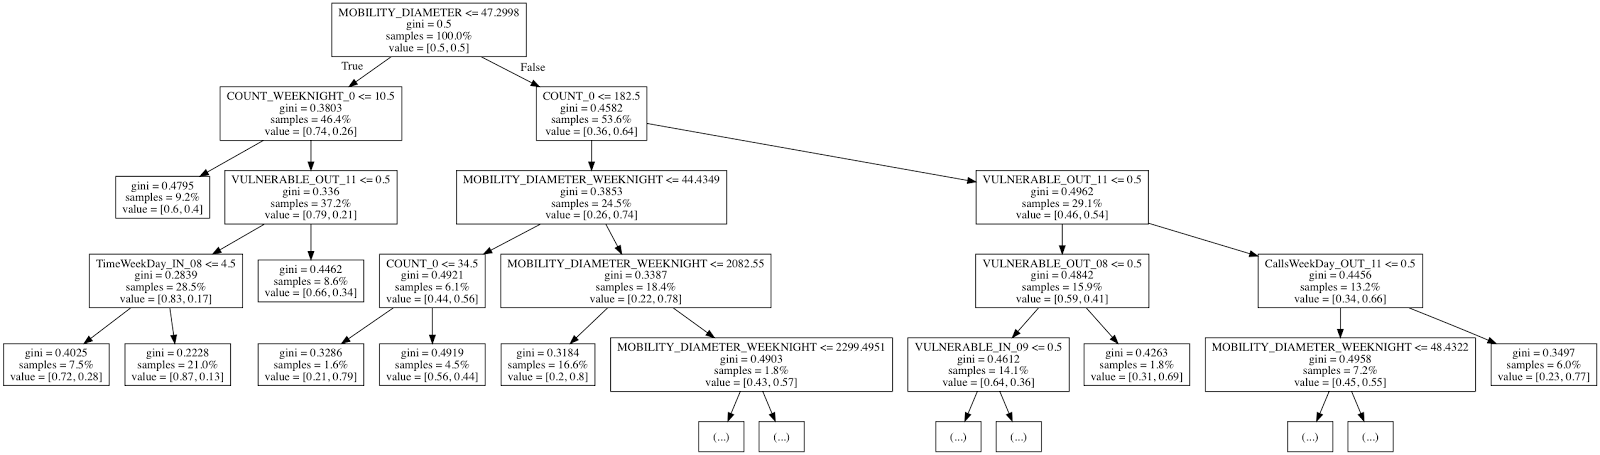
\includegraphics[width=.9\paperwidth]{figures/decision_tree/full_tree_map2.png}}
\caption{ Second example of a decision tree. This model was made with a cross validated procedure on \cref{target3} from an artificially balanced dataset. The resulting tree has been pruned to fit the image.}
\label{fig:decision_tree_actual_problem2}
\end{figure*}

\smallskip

From \cref{fig:decision_tree_actual_problem} the importance of the mobility diameter is more clear.
Once again the learner uses it as the first split in the data, even with balanced samples.
Recall that by the stochastic nature of the algorithm that builds a tree, two runs with the same setting need not output the same trees.
In this however, it is notable that the final tree still uses the mobility as the first split in the data, even with balanced samples.
And the same can be said of the feature representing the count of calls made from the home antenna.

This tree also performs poorly in its prediction of which users have migrated in the past.
At some point, it is reasonable to assume that balancing classes leads to a better predictive outcome.
Yet there are still various misclassifications in the predicted target classes.
If we let the tree grow deeper though, we might increase the performance of the training error as shown in \cref{figure:biasVariance}.
But again, this won't help our generalization error.
So to tackle most of the disadvantages described by this technique, \textit{Random Forests} are what follow as a natural extension to this classifier.


\section{ Random Forests}\label{section:random_forests}

Random Forests are estimators that extend from constructing a number of single decision trees and then combining them to produce a single output variable in what is called an \textit{ensemble}.
The objective in this construction is to focus on decision tree\'s low bias whilst controlling their overfit as much as possible.
The main idea behind this is that a forest of single trees will be constructed in such a way that correlations among each of the individual models is limited as much as possible.
The concept behind this is that each individual model will learn on a random subset of features or samples and then, an average of the single outputs will be used as the forest's target output.
In practice, there are other variants used to construct uncorrelated trees and then combine them, but the main idea still applies.

\subsection{ Random Forests Formulation}\label{subsection:random_forests_formulation}

Let $K$ be the number of trees in the ensemble and let $\Theta_k$ encode the parameters for the $k$-th tree.
As we have mentioned before, there are various variants to the model and these variants will define the type encoding of the $\Theta_k$ parameters.
For this part, we will not specify the type of ensemble constructed since the following proofs apply to all of them.

We denote $h(\textbf{x},\Theta_k)$ to be the corresponding classifier and $N$ the number of samples in the training set.
The creation of a random forest involves an iterative procedure where at the $k$-th step, the parameter $\Theta_k$ is fit from the same distribution but independently of the previous parameters $\Theta_1, \ \ldots, \ \Theta_{k-1}$. %$\Theta$ will be encoded by a vector of randomly drawn integers from 1 to $M$ which is part of the model's hyperparameters.


Let ${h_k(\textbf{x}) }_{i=1}^K$\footnote{There is an abuse of notation by noting trees as $h_k(\textbf{x})$ and not $h(\textbf{x}, \Theta_k)$ } be a set of classifying trees and let $I(\cdot)$ denote the indicator function.
Define the margin function as

\begin{equation}
mg(\textbf{x},\textbf{y}) = \frac{1}{K}  \sum_{k=1}^K I(h_k(\textbf{x}) = \textbf{y})
- \max_{j\neq \textbf{y}}\left(\frac{1}{K} \sum_{k=1}^K I(h_k(\textbf{x}) = j) \right)
\end{equation}\label{eq:rf-marginFun}


The margin function measures, in average, how much do the trees vote for the correct class in comparison to all other classes.
It is the training error of the model when using the misclassification loss. Here the generalization error is denoted as $PE*$ and is equal to

\begin{equation}
P_{\textbf{x}, \textbf{y} }(mg(\textbf{x},\textbf{y}) <0)
\end{equation}

 It can be shown that, for $K$ sufficiently large, the generalization error under the misclassification loss converges to

\begin{equation}
 P_{\textbf{x}, \textbf{y} } ( P_{\Theta} (h(\textbf{x}, \Theta) = \textbf{y}) - \max_{j \neq \textbf{y}} P_{\Theta} (h(\textbf{x}, \Theta) = j) < 0)
 \end{equation}

almost surely for all sequences of parameters $\Theta_1, \ldots, \Theta_k,\ldots$

\subsection{Proof}
The proof follows from seeing that given a training set, a tree $\Theta$ and a class $j$ then
\begin{equation}
\forall \textbf{x}  \ P_\Theta(h(\theta,\textbf{x}) = j) \ = \
\lim_{L\to\infty} \frac{1}{L} \sum_{l=1}^K I(h_l(\textbf{x}) = j) \
\end{equation}

almost surely.

This is because if we consider the nature of the tree, we see that the set $\{\textbf{x} / h_l(\textbf{x}, \Theta) = j \}$ is built as a union of hyper-rectangles partitioning feature space.
And given the finite size of the training set, there can be but a finite set of these unions of hyper-rectangles for all the input data.
Let $S_1, \ldots, S_M$ be an indexation of these unions and define $\phi(\Theta) = m $ if $\{\textbf{x} / h(\textbf{x}, \Theta) = j \} = S_m$.

We denote by $L_m$ the number of times that $\phi(\Theta_l) =m $, where $l \in {1,\ldots,L}$ and $L$ is the total number of trees in this forest.

It is immediate that

\begin{equation}
\frac{1}{L} \sum_{l=1}^L I(h_l(\textbf{x},\Theta) = j) \ = \ \frac{1}{L} \sum_{m=1}^M L_m I(\textbf{x} \in S_m)
\end{equation}\label{eq:rf-PEconvergence1}

and that following the law of large numbers, there is a convergence almost everywhere of
\begin{equation}\label{rf-PEconvergence2}
\frac{L_m}{L} = \frac{1}{L} \sum_{l=1}^L I(\phi(\Theta_l) = m) \xrightarrow[L \to \infty]{}  P_{\Theta}(\phi(\Theta)= m).
\end{equation}

If we let $C = $ $\bigcup\limits_{m=1}^{M} C_{m}$ where each $C_m$ are zero-measured sets representing the points where the sequence is not converging.
If we combine \cref{eq:rf-PEconvergence1} and \cref{rf-PEconvergence2}, we will finally have that outside of $C$,

\begin{equation}
 \frac{1}{L} \sum_{l=1}^L I(h_l(\textbf{x}) = j) \xrightarrow[L \to \infty]{} \sum_m^M  P_{\Theta}(\phi(\Theta)= m) I(\textbf{x} =j ) \ = \ P_{\Theta}(h(\textbf{x}, \Theta) = j)
 \end{equation}


\subsection{ Comparison to Decision Trees}\label{subsection:random_forests_comparison_trees}

From what is formulated in \cref{subsection:random_forests_formulation} and in order to compare how this model improves over the Decision Trees,  we ran two experiment setups on a Random Forest learner for the simple task in \cref{target1}, using an $F1$ score. This was a cross validation procedure of 10 folds for each configuration, where each experiment optimized the score on a different hyperparameter.

For the first one, we test the scores of the forest by varying the maximum depth that the trees can have.
And on the second one, we try to illustrate the point of \cref{subsection:random_forests_formulation} by considering forests of increasing tree size.
As a default configuration, we set on 10 the trees' max depth and on 10 the default number of trees.

In both, we set a balanced weighting of positive and negative samples in the loss function. Also, we use the Gini index as the impurity measure in the splitting criteria of each tree's node.

Cross validation procedures ran for 1412.8 and 2506.1 seconds respectively and they both excluded attributes of the user's which informed on the user's home state and its current endemic condition at $T_1$.

The experiment's scores outcomes across their hyperparameter values were graphed  in \cref{fig:f1_random_forest_validation_curves_depth_num_trees}.
The couple of cross-validated and training set scores where compared, where, for each hyperparameter value, the $1-F1$ score is shown.
In this way, having a lower score in the graphic means a better model was reached.

\begin{figure}
\centering
\begin{minipage}{.5\textwidth}
%  \centering
  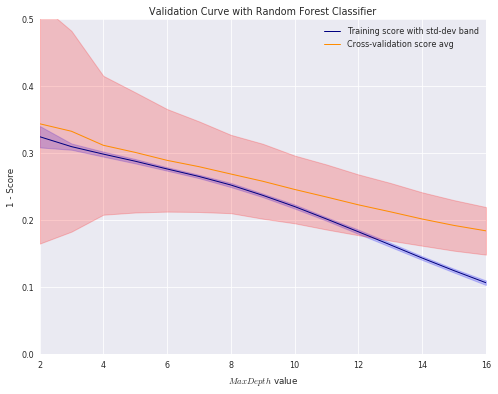
\includegraphics[width=.8\linewidth]{figures/random-forest/validation_curve_forest_depth_series_f1}
\end{minipage}%
\begin{minipage}{.5\textwidth}
%  \centering
  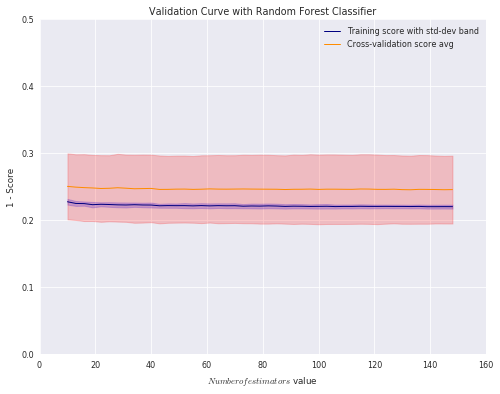
\includegraphics[width=.8\linewidth]{figures/random-forest/validation_curve_forest_num_trees_series_f1}
  \end{minipage}
\caption{ Side comparison of validation curves for two hyperparameters of the Random Forest learner. The mean CV scores for the $1 - F1$ score is shown where the number of trees and the depth of the trees hyperparameters were tested.}
\label{fig:f1_random_forest_validation_curves_depth_num_trees}
\end{figure}


Recall how this relates to \cref{figure:dtree_overfit_problem_2}, in which a tree's training error always improves as a result of an increase in the tree's depth.
Yet the tree's prediction error at one point suffers and deteriorates.
From what we can see in \cref{fig:f1_random_forest_validation_curves_depth_num_trees}, the cross validated error is always decreasing for increasing tree depth.
A very slight deceleration in the decrease of the cross validated error can be seen for tree depth bigger than 9.
Yet the scores keeps improving and don't worsen.
This is different to \cref{figure:dtree_overfit_problem_2} where if we let the tree grow deeper, at one point we only increase the performance of the training error.
Here, we are possibly improving the generalization error, as indicated by the CV estimation.

 On the other hand, it is interesting to note that there is a very slow decrease in the training and CV scores when the number of trees is increased.
 This might be explained by the fact that we are setting a default tree depth of 9 levels.
 A configuration of this type then might be capturing all the needed model complexity to attain
 Another plausible explanation for this is that, for this task, the forest rapidly converges to the generalization error and that adding more trees doesn't certainly improve on the predictions.


At their optimal configuration, both setups reached CV score averages of at least 0.75, with a maximum of 0.81 for the forest
with trees of 16 levels.
The optimal number of estimators for the CV and the training sets were not the same though, were 139 was the best configuration for the training score whilst 133 was the best average for the CV set. The relative difference in these best scores was of 3.3\%.
At the same time, the relative difference of the best CV and training scores, for the maximum tree depth experiment was of 9.5\%.
This percentage difference signals that the max depth hyperparameter is significantly more sensible to over-fitting than the number of trees parameter.


\subsection{Predictive error bounds}

Random Forests are built upon a bag of weaker classifier, of which each individual estimator has a different prediction error.
To build an estimate of the generalization error on the ensemble classifier, these individual scores and the relationship between them must be measured.
In this sense, the \textit{strength} and \textit{correlation}of a Random Forest must be analyzed to arrive on an estimate of the generalization error.

%\begin{lemma}
%Given two line segments whose lengths are $a$ and $b$ respectively there is a
%real number $r$ such that $b=ra$.
%\end{lemma}

\begin{theorem}
There exists an upper bound for the generalization error.
\end{theorem}


\begin{proof}
	Define $\hat{\jmath}( \textbf{x},\textbf{y})$ as $\argmax_{j \neq \textbf{y}} P_{\Theta}(h(\textbf{x}) = j)$ and let the margin function for a random forest (not a group of classifiers) be defined as

	\[\label{eq:rf-marginFunRf}
	mr(\textbf{x},\textbf{y}) = P_{\Theta}(h(\textbf{x}) = \textbf{y}) - P_{\Theta}(h(\textbf{x}) = \hat{\jmath})
	\\
	= \Expect_{\Theta} \left[ I(h(\textbf{x},\Theta ) = y ) - I( h( \textbf{x},\Theta ) = \hat{\jmath} ) \right]
	\]


	%\[%\]

	%\]

	Here the margin function is described as the expectation taken over another function which is called the \textbf{raw margin function}\label{eq:rf-rawMarginFun}.
    Intuitively, the raw margin function takes each sample to be $1$ or $-1$ according to whether the ensemble classifier can correctly classify or not the sample's label, given $\Theta$.

	With these definitions, it is straight to see that

        	%\[%\]
            \begin{equation}
            {mr( \textbf{x},\textbf{y} )}^2 = \Expect_{\Theta, \Theta'} \left[ rmg( \Theta,\textbf{x},\textbf{y} ) \ rmg(\Theta',\textbf{x},\textbf{y} ) \right]
            \end{equation}


	This in turn implies that
            \begin{equation}\label{eq:rf-marginFunVar}
	            \begin{split}
	            var(mr) & = \Expect_{\Theta, \Theta'}
	            \left[
	            cov_{\textbf{x},\textbf{y}}
	            (rmg(\Theta,\textbf{x},\textbf{y} )rmg(\Theta',\textbf{x},\textbf{y} ))
	            \right] \\
	            & = \Expect_{\Theta, \Theta'}
	            \left[
	            \rho(\Theta, \Theta')\sigma(\Theta)\sigma(\Theta')
	            \right]
	            \end{split}
            \end{equation}

	where $ \rho(\Theta, \Theta')$ is the correlation between $rmg(\Theta,\textbf{x},\textbf{y})$ and $rmg(\Theta',\textbf{x},\textbf{y})$, and $\sigma(\Theta)$ is the standard deviation of $rmg(\Theta,\textbf{x},\textbf{y})$.
    In both cases, $\Theta$ and $\Theta'$ are given.% to be fixed.

	Equation \cref{eq:rf-marginFunVar} in turn implies that

	\begin{equation}\label{eq:rf-varianceBound}
            \begin{split}
            var(mr) & = \overline{\rho} {(\Expect_{\Theta}\left[ \sigma(\Theta)\right] )}^2 \\
            & \leq \overline{\rho} \Expect_{\Theta} \left[ var(\Theta) \right]
            \end{split}
            \end{equation}

	where we have conveniently defined $\overline{\rho}$ as

	\begin{equation}\label{eq:rf-meanCorrelation}
            \frac{\Expect_{\Theta, \Theta'} \left[ \rho(\Theta, \Theta') \sigma(\Theta) \sigma(\Theta')\right]}
            {\Expect_{\Theta, \Theta'} \left[ \sigma(\Theta) \sigma(\Theta')\right]}
            \end{equation}

	Note that this is the mean value of the correlation.

	Let the strength of the set of weak classifiers in the forest be defined as

            \begin{equation}\label{eq:rf-strength}
            s = \Expect_{\textbf{x},\textbf{y}} \left[ mr(\textbf{x},\textbf{y} ) \right]
            \end{equation}

	Assuming that $s \geq 0$ we have that the prediction error is bounded by
            \begin{equation}\label{eq:rf-predictiveErrorBound1}
            PE^* \leq var(mr)/s^2
            \end{equation}
	by Chebyshev's inequality. On the other we also have that

            \begin{equation}\label{eq:rf-expectedVarBound}
            \begin{split}
            \Expect_{\Theta} \left[ var(\Theta) \right] & \leq \Expect_{\Theta} {\left[ \Expect_{\textbf{x},\textbf{y}}\left[ rmg(\Theta,\textbf{x},\textbf{y})  \right] \right]}^2 -s^2 \\
            & \leq 1-s^2
            \end{split}
            \end{equation}



	We can use \cref{eq:rf-varianceBound}, \cref{eq:rf-predictiveErrorBound1} and \cref{eq:rf-expectedVarBound} to establish the upper bound for the prediction error we are looking for

            \begin{equation}\label{eq:rf-PEBound}
            PE^* \leq \overline{\rho}\frac{(1-s^2)}{s^2}
            \end{equation}

\end{proof}


This bound on the generalization error shows the importance of the strength of each individual weak classifier in the forest and the correlation interdependence among them. The author of the algorithm~\cite{breiman-randomforests} remarks here that this bound may not be strong. He also puts special importance on the ratio between the correlation and the strength $\frac{\overline{\rho}}{s^2}$ where this should be as small as possible to build a strong classifier.


\subsection{Binary Class}\label{subsection:random_forests_binary_class}

In the context of a binary class problem, where the target variable can only take two values, there are simplifications to the formula \cref{eq:rf-PEBound}. In this case, the margin function takes the form of $2 P_{\Theta}(h(\textbf{x}) = \textbf{y}) -1$ and similarly the raw margin function results in $2 I(h(\textbf{x}, \Theta) = \textbf{y}) -1$.


The bounds prediction error bounds derived in \cref{eq:rf-predictiveErrorBound1} assume that $s >0$ which in this case results in
\begin{equation}
\Expect_{\textbf{x},\textbf{y}} \left[ P_{\Theta}(h(\textbf{x}) = \textbf{y}) \right] > \frac{1}{2}
\end{equation}


Also, the correlation between $I(h(\textbf{x}, \Theta) = \textbf{y})$ and \ $I(h(\textbf{x}, \Theta') = \textbf{y})$, denoted $\overline{\rho}$ will take the form

\begin{equation}
 \overline{\rho} = \Expect_{\Theta,\Theta'} \left[ \rho \left( h(\cdot{},\Theta) ,h(\cdot{},\Theta') \right)  \right]
 \end{equation}



%


\subsection{Other Notes on Random Forests}\label{subsection:random_forests_other_notes}

One benefit of building Random Forest classifiers is that the algorithm easily increases the prediction error of a group of estimators by randomly building each of these in a way that decreases the variance of the overall model whilst trading a small loss in bias. The model is also robust to the introduction of a number of noisy features. If the ratio of informative to non-informative features is not extreme, selecting $m$ features at random at each split will mean that in most cases, splits will be made on those informative features. Note that in any given tree, the probability of drawing at least one informative feature in a split is still very high. This is because it follows a hyper geometric distribution $\mathcal{H}(P,j,l)$ with $l$ draws from a total population of $P$ features and only $j$ informative ones.

The depth of growth for each tree is another important tuning parameter. We must chose it correctly by assessing the model's performance across different values for $m$. A deep tree will tend to overfit the data by partitioning input space to fit the training data. This effect will counter the overall reduction in variance of the forest and thus increase the generalization error of our algorithm.

%Therefore controlling the maximum allowed growth for the base learners will be important to improve the performance of the model.

The algorithm also benefits from a heuristic to measure variable importance, where a special modification in the way forests are built allows this to happen.
The idea for this is that at each split we can measure the gain of using a certain variable for the split versus not using it. Given a candidate feature $X_j$ to be analyzed and for every node in a tree where a split is to be done, we compare the improvement in the split performance, as measured by some loss function, with and without $X_j$.
These results are recorded and averaged across all trees and all the split scenarios to have a score for the feature.
With this, the features with highest scores can be thought to be the most informative variables of the model.

\subsection{Experiments}\label{subsection:random_forests_experiments}

In this subsection, we explore on the task described on \cref{target4} by fitting random forest learners.
Here, our cross validation procedure explored multiple combinations of hyperparameters that we predefined Let $\alpha_i \forall i \in {1,\ldots,j}$ be the list of our $j$ hyperparameters.

Denote all possible combinations by $A_1 \times A_2 \ldots \times  A_j$, where each hyperparameter $\alpha_i$ will take all possible values in the predefined sets $A_i$.
In practice, we must be careful with the size of these combinations since the full cross validation procedure is costly for the Random Forest algorithm.
The learner has $j \geq 10$ and for each $A_i$ it is normal to have more than 10 possible values.
Thus the search will span a space of more than ten thousand combinations.
Moreover, each combination has to be cross validated on the number of folds we define, creating a very large amount of iterations during this search.
These fits will take computer resources such as memory and CPU time.
So we have to limit ourselves to search over a limited amount of values.

Also, if we were to use commodity hardware with standard tools for this procedure, the experiment would take weeks and, given our dataset size, it would not fit into a standard computer's memory of less than 12GB of memory.

For these reasons, we take on the task with a specialized server with a 16 core CPU and 72 gigabytes of available RAM.\@
The system runs a UNIX based OS and our algorithms were scripted in~\cite{python3.5}.
We used the specialized machine learning package~\cite{graphlab} to handle the parallelization and the distribution of system resources.
As a side note, we can't stress enough how convenient this package is for our purposes.
It handles most of the complex task of maxing out the system resources to perform as fast as possible in the cross validation procedure and in the construction of the main $X$ dataset.
Also, it has an \textit{out-of-the-box} memory management for large datasets.
With this, we can natively handle data that is larger than the amount of memory used by the server, requiring minimal user knowledge to tune.
\cite{graphlab} has allowed us to conveniently run these long experiments without risk of failure due to lack of memory and without any prior expert domain knowledge in multi-threading or parallel computing.

For this case, we only considered migrant people that are non-endemic at $T_1$, but have been during $T_0$.
In the general procedure, we cross validated the same possible hyperparameter configurations, where these spanned the following items:

\begin{itemize}\label{list:random_forest_grid_search_params}

  \item Every tree's maximum depth --- [max\_depth]
  \item If the loss function will balance the weights of the positive and negative classes --- [balanced]
  \item The maximum number of trees to grow in each fit--- [max\_iterations]
  \item The splitting criterion at each node which can be either by the Gini Index or the Entropy condition--- [split\_criteria]
  \item The sample percentage of features which are available to use at each split --- [max\_features]
  \item The minimum number of samples required to split a node --- [min\_split]
  \item The scoring function used to evaluate the learner in the CV evaluation --- [CV score]
  \item The minimum reduction in the loss function required to split a node  --- [min\_loss]
%\caption{Available hyperparameters for the Random Forest classifier, with their corresponding code names.}
\end{itemize}


The full experiment ran two different tasks, where each was characterized by the attributes used for our $X$ dataset.
In the first one, the procedure ran with all available features and in the second one we separated the features that had a high correlation, bigger than $0.3$, with the target variable.
This means we removed all of the features that counted the user\'s vulnerable neighbors for a given month, segmented by the direction of the call.\footnote{For a complete description on the definition of these features, please refer to \cref{tab:data_example}.}
Recall that all of these features were central in the construction of the risk maps in \cref{section:riskmaps}.
The color of each antenna's circle represented the amount of vulnerable users, for that given month, when looking at the incoming or outgoing calls.
Then, these feature's correlation to the target variable are indicative, up-to a certain point, of the predictive power of them.

For this experimentation, we recorded the outcome of the cross validation procedures in terms of different scoring metrics, the runtime, the hyperparameters chosen and the top ten best features as given by the algorithm. The summary of these results is given in \cref{tab:random_forest_big_experiment_results}.

\begin{table}[!htb]
\caption{Table of best results comparing two 5-fold full grid cross validation procedures on a Random Forest Classifier.  The metrics and runtime for both experiments are shown.}
\label{tab:random_forest_big_experiment_results}
\centering
\begin{tabular*}{0.9\textwidth}{@{\extracolsep{\fill} }  l l l l l }
%{|p{2cm}|p{2cm}|p{1.5cm}|p{1cm}|p{1.5cm}}
\toprule
Result & Experiment 1 & Experiment 2 \\
\midrule
CV $F1$ score           & 0.770  &  0.663 \\
CV $Accuracy$ score    & 0.848 &  0.843 \\
CV $Precision$ score    & 0.788 &  0.780 \\
CV $Recall$ score       & 0.753 &  0.557 \\
CV $Logloss$ score     & 0.391 &  0.337 \\
CV $ROC AUC$ score     & 0.903 & 0.880  \\
max\_depth     & 12 &  12 \\
max\_iterations          & 150 &  200 \\
balanced        & True & True  \\
split\_criteria          & Gini &  Gini \\
min\_loss  & 10 &  1 \\
Running time (s)        & 2030 &  2064 \\
 max\_features (\%) & 50 & 80  \\

\bottomrule
\end{tabular*}
\end{table}


From the result's table, it's relevant to note that both optimal learners chose the Gini splitting criterion as best, with tree's of a relatively high depth with 12 levels.
A similar situation happened with the number of trees grown; best configurations had more than 100 trees with the second experiment having an optimal number of 200.

Bigger differences appear in the choice of the minimum loss reduction and the features sampled per split.
There are no clear indications as to which configuration is better.
And, whilst having a higher level of randomization in the growth of the trees hints to a less overfitting learner, this difference is not that notable in the CV scorings.

For most of the metrics used to evaluate the cross validation procedure, the scores look very similar. It is notable that the second experiment is slightly better in the accuracy, precision, logloss and ROC AUC scores, with a maximum difference of 5\% for all of them.
Yet at the same time the second experiment's performance drastically drops for the recall and, because of this, for the $F1$ measure.
This means that the learner is losing performance in correctly tagging the user's who have migrated from the endemic region.
This 15\% difference hints to how much of an impact is characterized by removing the features for the second experiment.
We can suspect that there's enough missing information in those features to reduce the predictive power of the learner.

In both experiments, its important to note though that the elected hyperparameters are not optimal in any strict sense.
At most, they can hint to the best possible configuration.
Given the large combinatorial nature of this process, there is no guarantee of optimality in this search.
To a greater degree were only covering as much space as our time and our computational systems allow.


We also recorded the model's selection of best features, using the explanation outlined in \cref{subsection:random_forests_other_notes}.
This outcome is presented in \cref{tab:random_forest_big_experiment_best_features}, where the top 10 features for each experiment are shown.

\begin{table}[ht]
    \centering
    \resizebox{\textwidth}{!}{%
        \begin{tabular}{@{}llll@{}}
            \toprule
            & \multicolumn{3}{l}{Top Features}                                                                   \\ \midrule
            \multicolumn{1}{l|}{\multirow{4}{*}{First Experiment}}  & Call Count Antenna\_0    &   Mobility Diameter   & Mobility Diameter Weeknight \\
            \multicolumn{1}{l|}{}                                   & Call Count Weeknight Antenna\_0 & TimeWeekDay Out Month\_09       & CallsWeekDay In Vuln Month\_08 \\
            \multicolumn{1}{l|}{}                                   & TimeWeekDay Out Month\_08       & State Hidalgo          & CallsWeekDay In Month\_08      \\
            \multicolumn{1}{l|}{}                                   &                                 & TimeWeekDay Out Month\_12       &      \\ \midrule
            \multicolumn{1}{l|}{\multirow{4}{*}{Second Experiment}} & Mobility Diameter               & Call Count Antenna\_0           & Mobility Diameter Weeknight    \\
            \multicolumn{1}{l|}{}                                   & Call Count Antenna\_1           & Call Count Weeknight Antenna\_0 & TimeWeekDay Out Month\_12      \\
            \multicolumn{1}{l|}{}                                   & TimeWeekDay In Vuln Month\_09   & TimeWeekDay Out Vuln Month\_08  & TimeWeekDay Out Month\_09      \\
            \multicolumn{1}{l|}{}                                   &                                 & TimeWeekDay In Vuln Month\_08   &                                \\ \midrule
        \end{tabular}%
    }
    \caption{A representation of the top features that resulted from the Random Forest experiment on \cref{target4}. }\label{tab:random_forest_big_experiment_best_features}
\end{table}


The top features list shows us the importance of mobility diameter in both cases.
Where for weeknights and for the whole week, the user's mobility is  relevant to detect his past endemic condition.
As expected, in both cases we see that there are a number of features logging vulnerable interactions of users living in non-endemic regions.
This is in line with what we hypothesized in the construction of the risk maps in \cref{section:riskmaps}.
The direction of the call and the calls' duration or number of occurrences are both important predictors of this model.
Given that this best feature methodology is an heuristic, there doesn't seem to be any clear indication over which type of CDR interaction has better predictive power.
Yet there is a preference for interactions logged in the earlier months, August and September,
This might be the case where the algorithm is picking up on the most recent migrations, given that our time period of analysis $T_1$ starts in August.

The analysis here presented is relevant in answering the question of long-term migrations.
High scores for these experiments show that there is value in CDR data to predict long-term migrations between two regions.
Also, top features are in line with the assumptions on which the risk maps were constructed.



\section{Boosting Models}\label{section:gradient_boosting}

Boosting methods are similar to additive methods such as in Random Forests because they combine the predictions of weak learners to output the combined model's prediction.
The full model is grown sequentially from base estimators such as decision trees, but the difference is that each new iteration tries to reduce the overall bias of the combined estimator.
This provides greater predictive power when the base model's accuracy is weak. But care must be taken to control the increase in variance.

\subsection{Ada Boost}
%~\cite{schapire-adaBoost}

In the Ada Boost variation of ensembling, each iteration builds a new weak learner which is set to improve on the samples misclassified by the weak learner before, rather than building a new uncorrelated learner.
Weights are used to rank the samples by importance, where a sample with higher misclassification rate will receive a stronger weight.
The name of the algorithm is derived from the term \textit{adaptive boosting}, where sample weights are updated at each iteration.

Tuning parameters in this algorithm are the same as those in the base learners. In addition, the number of steps that the algorithm will \textit{boost} is a new hyperparameter.

The chained construction of weak learners has its implications in computational complexity. Base learners are not constructed independently and as such, the parallelization of this algorithm is rarely possible. At the same time, the sequential optimization of learners improving on the one before marks a \textit{greedy} minimization approach of the general loss function.

These properties underline a substantial difference to Random Forests where base learners are built as uncorrelated as possible and where optimization can be performed globally, which allowed a significant parallelization of the algorithm.

\subsection{Ada Boost Formulation}\label{subsection:gradient_boosting_formulation}

Let
\begin{equation}\label{eq:adaBoostTrainingError}
\overline{err} = \frac{1}{N} \sum_{i=1}^{N} I(y_i \neq \hat{y_i})
\end{equation}

denote the training set's misclassification error. As usual, $N$ is the amount of samples in our dataset, $y$ is our target variable and $\hat{y}$ is our model's prediction for the target, given the samples. We also take
\begin{equation}
\Expect_{X \ Y} [ I(Y \neq \hat{Y}(X)) ]
\end{equation}

to be the expected error rate of the model on the true, unknown distribution of the data.

Let $m$ index the iteration number in the Ada Boost algorithm. Set $w^{(m)}_i$ to be the $i$-th sample's weight. We will initialize this variable to be equiprobable at $w^{(0)}_i = \frac{1}{N} \forall i$. Let $h(x,\theta)$ denote our model's weak learner. With this notation, we assume the function to have a domain in the input feature space and in the parameters defining the learner. Naturally these will depend on the problem structure and on the base learner. Then Ada Boost's model takes the following form:

\begin{equation}\label{eq:adaBoostModel}
\hat{y}(x) = \sum_{m=1}^{M} \gamma_m h(x,\theta_m)
\end{equation}

where $M$ is the model's hyperparameter indicating the amount of weak learners and thus the amount of iterations. Here, each $\theta_m$ will encode the base learner's parameters and $\gamma_m$ will denote the weight of that weak learner in the overall model.

The algorithm's iteration will build $\hat{y}$ starting from $\hat{y_i}^{(0)}= 0 \forall i$ and at each stage we will minimize a function that tries to correct the performance of the last model. At step $m$ we will search for $(\gamma_{m}, \theta_{m})$ where

\begin{equation}\label{eq:adaBoostIteration}
\begin{split}
(\gamma_{m}, \theta_{m}) = \underset{\gamma, \theta}{\mathrm{argmin}} \sum_{i=1}^{N} & L\big( y_i,  \hat{y}^{m}(x_i) + \gamma h(x_i,\theta) \big) \\
= \underset{\gamma, \theta}{\mathrm{argmin}} \sum_{i=1}^{N} & L\big( y_i,  \sum_{j=1}^{m} \gamma_j h(x_i,\theta_j) + \gamma h(x_i,\theta) \big)
\end{split}
\end{equation}

The greedy nature of the algorithm becomes explicit in the procedure above, where we have fixed all the previous optimized values for $\gamma_j$ and $\theta_j$.

Ada Boost was first derived in~\cite{schapire-adaBoost} and it was introduced with a specific minimizing function. The general version here presented allows the use of a broad range of base learners which need not to be from the same algorithmic family. In the first version introduced, the loss function used was the exponential loss which is $L(y,z) = e^{-yz}$ and the target variable took the values $1$ or $-1$.

This particular case yields a similar equation as in \cref{eq:adaBoostIteration}, but where

\begin{equation}\label{eq:sadaBoostExponentialIteration}
\begin{split}
(\gamma_{m}, \theta_{m}) = \underset{\gamma, \theta}{\mathrm{argmin}} \sum_{i=1}^{N} & \exp\big( -y_i (\hat{y}^{m}(x_i) + \gamma h(x_i,\theta) )\big) \\
= \underset{\gamma, \theta}{\mathrm{argmin}} \sum_{i=1}^{N} &
\exp\big( -y_i \hat{y}^{m}(x_i)\big) \exp\big(- \gamma h(x_i,\theta)y_i \big)
\end{split}
\end{equation}


Given that we are only minimizing $\gamma$ and $\theta$, we can group $e^{-y_i \hat{y}^{m}(x_i)}$ into a single value $w_i^{(m)}$ which we will set to the weight of each sample. This weight strongly depends on the past steps of the algorithm. The equation now becomes

%We can also take the $\gamma$ factor out of the sum, since it is fixed for all samples.
*
\begin{equation}\label{eq:adaBoostExponentialIteration2}
(\gamma_{m}, \theta_{m}) = \underset{\gamma, \theta}{\mathrm{argmin}} \  \sum_{i=1}^{N} w_i^{(m)} \exp \big(-\gamma h(x_i,\theta)y_i \big)
\end{equation}

We can then minimize for $\theta$ first, independently of the value of $\gamma$. The series in \cref{eq:adaBoostExponentialIteration2} can be decomposed

\begin{equation}\label{eq:adaBoostThetaDecomposition}
\begin{split}
e^{-\gamma} \sum_{i \mid y_i = h(x_i,\theta)} w_i^{(m)} + e^{\gamma} \sum_{i \mid y_i \neq h(x_i,\theta)} w_i^{(m)} & = \\
( e^{\gamma} - e^{-\gamma}) \sum_{i = 1}^{N} w_i^{(m)} I \big( y_i \neq h(x_i,\theta)  \big) + e^{-\gamma} \sum_{i = 1}^{N}  w_i^{(m)} &
\end{split}
\end{equation}


and then the minimizing solution for $h(\cdot, \theta_{m+1})$ will be the one satisfying

\begin{equation}\label{eq:adaBoostThetaMinimization}
\theta_{m} = \underset{ \theta}{\mathrm{argmin}} \sum_{i=1}^{N} w_i^{(m)} I \big( y_i \neq h(x_i,\theta)  \big)
\end{equation}

Let $u = \sum_{i=1}^{N} w_i^{(m)}$ and $v = \sum_{i=1}^{N} w_i^{(m)} I \big( y_i \neq h(x_i,\theta)  \big) $, which are both constant in $\gamma$. Consider \cref{eq:adaBoostTrainingError} and note that $\frac{u}{v} = \frac{1}{\overline{err}}$. If we now solve for $\gamma$ in \cref{eq:adaBoostThetaDecomposition}, we can take

\begin{equation}\label{eq:adaBoostBetaMinimization}
f(\gamma) = ( e^{\gamma} - e^{-\gamma}) u + e^{-\gamma}v
\end{equation}

which has a minimum at
\begin{equation}
\gamma_{m} = \frac{1}{2} \log\big( \frac{1 - \overline{err} }{ \overline{err} } \big)
\end{equation}

As seen from the equation above, the minimizing value for $\gamma$ is directly related to the training error of the algorithm for the \textit{whole} dataset. This weight will be reflected upon all samples in general and then we would expect this rate to decrease at every iteration. Taking advantage of this closed form, the value is plugged into the next step of the Ada Boost procedure to update sample weights as

\begin{equation}
w_i^{(m+1)} =  w_i^{(m+1)} e^{\gamma_m(-y_i h_m(x_i))} \\
\end{equation}

In this way, we have that the weights are updated for those samples which have a higher misclassification rate. This is a relevant aspect of the algorithm. At each step, more importance is given to misclassified samples over correctly classified ones.

%$-y_i h_m(x_i) = 2I \big( y_i = h_m(x_i)  \big) -1$ which means that $\gamma_m(-y_i h_m(x_i))$


The final form of the model is
\begin{equation}
 \hat{y}(x) = sgn\big( \sum_{m=1}^{M} \gamma_m h_m(x) \big)
\end{equation}
  which outputs the most frequent prediction given by all of the weak learners. This is because all the correct predictions will be greater than zero and negative values for the incorrect predictions.\footnote{This is when we consider the binary class case where $Y$ can take only $1$ or $-1$ values.}
%This particular property is what gives rise

At first the choice of the exponential loss function can seem arbitrary, but in the context of statistical learning this measure presents an important property where its minimizing function is the log-odds ratio of the two output classes:
\begin{equation}
f^*(X) = \underset{f}{\mathrm{argmin}} \ \Expect_{Y | f(X)}\big[ \exp(-Yf(X)) \big] = \frac{1}{2}\log\big( \frac{ P(Y=1 \mid X) }{ P(Y=-1 \mid X) } \big)
\end{equation}


The use of the exponential loss function $\exp(-Yf(X))$ is also desirable in this context since significantly more weight is put on misclassifications rather than on correct classifications. This is because the function is not symmetric in $Yf(X)$ and that having a correct classification will mean a factor of only $e^{-1}$, whilst on the other hand a misclassification will mean a factor of $e$.

A drawback of this loss though, is that it is not robust to outliers or to noisy data. During runtime weights are constantly shifting towards misclassified samples. Then if samples are mislabeled, this will make the algorithm repetitively focus on classifying incorrectly the data.


\subsection{ Comparison to Random Forests}\label{subsection:boosting_comparison_forest}

In order to compare this learner to Random Forests, we ran the same setup as in \cref{subsection:random_forests_comparison_trees}
with two experiments each varying a different hyperparameter.
The Boosting models were built to classify on task \cref{target1} and the $F1$ score was used to evaluate their performance.
The cross validation procedure set 10 folds for each hyperparameter
 configuration and both experiments individually tuned on: a) the maximum tree depth and b) the number of base learners.

For both, we vary the tested hyperparameter's values over a predefined range and then graph the change in score across these values.
As a default configuration, 50 was the number of trees, and 6 were the trees' maximum depth and 0.1 was the fixed learning rate.
Additionally, we used the Gini index as the impurity measure in the splitting criteria of each tree's node and the exponential loss function to grow the next estimator in line with the formulation given in \cref{eq:adaBoostThetaDecomposition}.
% .\footnote{Other loss functions are available but these would not yield the AdaBoost formulation.}

Cross validation procedures ran for 82150.8
 and 6076.3 seconds respectively and they both excluded attributes of the user's home state and their current endemic condition at $T_1$.

The experiment's scores outcomes across their hyperparameter values were graphed in \cref{fig:f1_boosting_validation_curves_depth_num_trees}.
These compare the cross-validated and training set scores, where, for each hyperparameter value, the $1-F1$ score is graphed as a function of the hyperparameter's value.
In this way, having a lower score in the graphic means a better model was reached.

\begin{figure}
\centering
\begin{minipage}{.5\textwidth}
%  \centering
  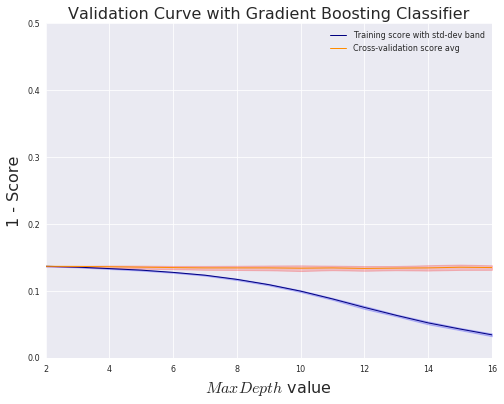
\includegraphics[width=.8\linewidth]{figures/gradient-boosting/validation_curve_boosting_depth_series_f1}
\end{minipage}%
\begin{minipage}{.5\textwidth}
%  \centering
  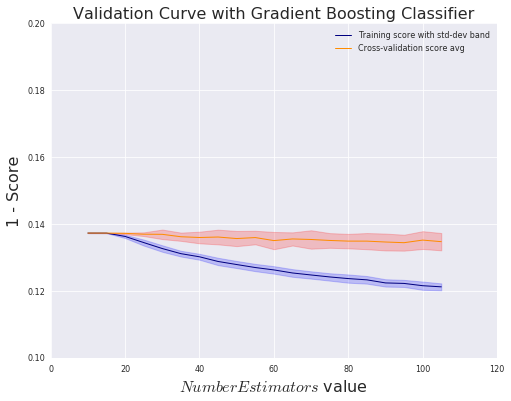
\includegraphics[width=.8\linewidth]{figures/gradient-boosting/validation_curve_boosting_num_trees_series_f1}
  \end{minipage}
\caption{ Side comparison of validation curves for two hyperparameters of the Gradient Boosting learner. The mean CV scores for the $1 - F1$ score is shown, where the number of trees and the depth of the trees hyperparameters were tested in separate experiments.}
\label{fig:f1_boosting_validation_curves_depth_num_trees}
\end{figure}


Recall how these outcomes compare to \cref{figure:dtree_overfit_problem_2} and \cref{fig:f1_random_forest_validation_curves_depth_num_trees},
in which a tree's training error always improves as a result of an increase in the tree's depth.

Here, we see that the estimator is prone to overfitting when using a high $max depth$ value.
This is because the training deviates faster from the CV error when the depth is higher.
This acceleration is clear from the figure where the CV score is invariant while the training error decreases.
This model differs to the Random Forest classifier in that the trees are not uncorrelated, because the $t$-th tree improves on the error of the model at $t$.
This is an effective difference in the models.

For the second experiment, the overfitting difference in the CV score and the train score is smaller, relative to the CV score.

It is interesting to note that, for both cases, there is a very small gain in the CV error when varying the hyperparameters, as evidenced by the range of the scores.
Yet the decrease in CV score is slightly better for the second experiment.
This is different to the Random Forest experiment, where the scores had a stronger improvement in the cross validated score.
The learner seems to better fit the data than the Random Forest model, since lower error rates are achieved, and it converges faster to a stable CV error where adding more trees or depth doesn't improve on the score.

At their optimal configuration, both setups reached CV score averages of at least 0.865, with a maximum of 0.8659 for the learner with trees of 12 levels.
However, the optimal number of estimators for the CV and the training sets were different, were 105 was the best configuration for the training score and 95 was the best average for the CV set. The relative difference in these best scores was of 1.5\%.
It is not surprising that the relative difference of the best CV and training scores, for the maximum tree depth experiment was much higher, with 11.5\%.

The outcomes here expose the drawbacks of this model which is more prone to overfitting and takes longer to fit when compared to the Random Forest algorithm.
Yet it gives better overall performance on the CV error, when the model is correctly calibrated.



\subsection{Gradient Tree Boosting}

\todo{Add reference to Friedman paper in "Friedman-gradientBoosting2001"}

As explained before, the boosting method builds a high model learned from other \textit{weaker} learners. In the case of \textit{gradient tree boosting}, decision trees serve as base learners. If $Tr$ is a set of tree models and $K$ the number of trees in $Tr$, then trees will be the parameters for this model and at step $m$ the output will be

\begin{equation}
\hat{y}^{(m)}= \sum_t^m \gamma_t h_t(x) , \ h_t \in Tr \ \forall t \in {0,\ldots,K}
\end{equation}

where $\gamma_t$ indexes the weight for each tree $h_t$ and $K$ is a hyper-parameter that represents the number of trees. Each new base learner is added to the model

\begin{equation}
\hat{y}^{(m+1)} =  \hat{y}^{(m)} + \gamma_m h_m(x)
\end{equation}

and the latest base model is selected upon minimizing the misclassification rate of the full model in the previous step $m$, where a loss function previously selected is minimized to select the next best base learner:

\begin{equation}
h_m(\cdot) = \underset{h,\gamma}{\mathrm{argmin}}  \sum_{i=1}^{n} L ( y_i, \hat{y_i}^{(m-1)} - \gamma h(x_i) )
\end{equation}


For the moment, we include the tree's weight $\gamma$ as part of the weak learners in a single function $f_t(\cdot)$. Therefore the model results in,

\begin{equation}
y = \sum_k f_t(x) , \ f_t \in Tr \ \forall t \in {0,\ldots,K}
\end{equation}

where we represent a single tree with the form

\begin{equation}
f(x) = \theta_{q(x)} = \sum_{j=1}^J \theta_j I(x \in R_j)
\end{equation}

with $\theta_j \in \mathbb{R} \ \forall j = 1,\ldots,J$ and $ \cup_{j=1}^J R_j$ a partition of feature space. The function $q : X \mapsto \{1,\ldots,J\}$ denotes the mapping from samples to regions. In summary, ${\{\theta_j, R_j\}}_{j=1}^J$ are the weak model's parameters and $J$ is a hyper-parameter. Note that finding the best partition of feature space is a non-trivial optimization problem since finding subset partitions satisfying a global condition is a combinatorial feat.

For the high model, the objective function would account for the relationships among the trees and we would have that

\begin{equation}
Obj(\Theta) = \sum_i^n l(y_i,\hat{y}_i) + \sum_t R(f_t)
\end{equation}\label{eq:boositing-objfunction}\footnote{In the formula \cref{eq:boositing-objfunction} }

At this level $\Theta$ is a parameter encoding all of the base trees' model information. For each base tree $f_t$, $\theta_t$ is the parameter associated to it. This means that $\Theta = \bigcup_{t \in {0,\ldots,K}} \theta_t \cup \theta_0$. The parameter $\Theta_0$ is not associated to any tree but reserved to characterize the tree ensemble.

If an optimization routine were to collectively fit all the parameters in $\Theta$ to learn this model, we would have a very computational complex model. In practice this would result in an prohibitive cost. Instead, we rely on optimization heuristics.

\subsubsection{Additive Training}

As usual, the first take on this optimization problem goes using a greedy optimization routine. One tree is fit at a time and new trees are then successively added in later steps to improve on previous trees' errors.

Let $t$ be the step indexer of the algorithm, where $t \in {0,..,K}$, $Obj_t(\Theta)$ be the objective function and $\hat{y}^t$ be the target variable respectively. Then the $i$-eth target's value at each step would iterate in the following way:

\begin{equation}\label{eq:gb-targetSteps}
\begin{split}
\hat{y}_i^0 = & 0 \\
\ldots \\
\hat{y}_i^t = &\sum_{k=1}^{t} f_k(x_i) = \hat{y}^{t-1}_i + f_t(x_i)
\end{split}
\end{equation}
%\sum_{i=0}^{\infty} a_i x_i
where each tree is added in such a way that we are minimizing

\begin{equation}
Obj^t(\theta) = \sum_i^n L(y_i, \hat{y}^{t-1}_i + f_t(x_i) ) + c(t) + R(f)
\end{equation}


Note that we have included here a regularization term (see section \cref{section-hyperParametersRegularization}) $R$ on all of the weak learners. For most cases, this term will be in the form of a Tikhonov regularization. This will add another complexity tuning parameter to control the length of the overall procedure $c(t)$ which is variable only in $t$.

If we assume we have sufficient conditions to approximate the objective function with second order Taylor approximation around $f_t(x_i)$,we would have

\begin{equation}\label{eq:gradientBoostingTaylor}
Obj^t(\theta) \approx \sum_i^n {L(y_i, \hat{y}^{t-1}_i) + g_i f_t(x_i,\theta_t) + \frac{1}{2} h_i {f_t(x_i,\theta_t)}^2 } + R(f(\Theta)) + c(t)
\end{equation}

Here $g_i$ and $h_i$ are first and second order approximations of the loss function with,

\begin{equation}
\begin{split}
g_i = & \frac{\partial L(y_i, \hat{y}^{t-1}_i)}{\partial \hat{y}^{t-1}_i},  \\
h_i = & \frac{\partial^2 L(y_i, \hat{y}^{t-1}_i)}{\partial {(\hat{y}^{t-1}_i)}^2 }
\end{split}
\end{equation}

Still, the equation \cref{eq:gradientBoostingTaylor} can be simplified by taking only the terms that are dependent on $\theta$. This also means replacing the actual tree's predictions for each sample as $\theta_{q(x_i)}$, where $q(\cdot): X \rightarrow leaf$ is the function that maps samples to the tree's leaves. Then,

%for that tree's evaluation.

\begin{equation}\label{eq:gb-objSteps1}
Obj^t(\theta) \approx \sum_i^n {g_i \theta_{q(x_i)} + \frac{1}{2} h_i \theta_{q(x_i)}^2 } + \gamma ({t-1}) + \frac{1}{2}\lambda \sum_{j=1}^{t-1} \theta_j^2 \\
\end{equation}

As an example, we have already replaced the regularization terms $c(t)$ and $R(f)$ with penalties on the size of the ensemble and with an $l$2 penalty on the weight of each individual leaf.

If we rearrange the equation above we get

\begin{equation}\label{eq:gb-objSteps2}
\begin{split}
Obj^t(\theta) \approx & \sum_{j=1}^{t-1} \left( \sum_{i \in \{q(x_i)=j\}} (g_i )\theta_{j} + \frac{1}{2} \sum_{i \in \{q(x_i)=j\}} (h_i + \lambda ) \theta_{j}^2 \right) + \gamma ({t-1}) \\
\approx & \sum_{j=1}^{t-1} \left( \theta_{j}\sum_{i \in \{q(x_i)=j\}} (g_i ) + \frac{\theta_{j}^2}{2} \sum_{i \in \{q(x_i)=j\}} (h_i + \lambda ) \right) + \gamma ({t-1})
\end{split}
\end{equation}

which, as a function of $\theta$ is a quadratic equation if we assume $\gamma$ to be fixed. This results in a convenient and closed-form analytical formulation to select the value at step $t$. In this sense, a greedy direct optimization approach, such as gradient descent, can be used to find the tree $f_t(\theta)$ minimizing the previous expression.

As we have stated before the approach assumes that we have met enough smoothness conditions on the loss function with respect to the prediction variable
%$ \forall i \in {1\ldotsn}, \forall t \in {1..K}, \exists g_i(\hat{y}^{t}_i), h_i(\hat{y}^{t}_i) $
and that these values are actually computable. This is why smooth loss functions play an important part here in providing a feasible method.

%\begin{equation}

%Obj^t(\Theta) \approx \sum_i^n { g_i f_t(x_i) + \frac{1}{2} h_i f_t(x_i)^2 } + Obj_{t-1}(\Theta) + R(f_t) - R(f_{t-1})
%\end{equation}

%This equation form results in a direct method for a greedy optimization approach. We will have to search for the tree $f_t$ that minimizes \\
%$\sum_i^n { g_i f_t(x_i) + \frac{1}{2} h_i f_t(x_i)^2 } + R(f_t)$ at the $t$-th step.


As a concluding remark on boosting algorithms, there are two additional heuristics used to improve the generalization performance of boosting algorithms. The arguments in favor of these methods are rather experimental and not much theoretical, although their benefits are intuitive. The authors in~\cite{hastie-elemstatslearn} and~\cite{bishop-patternRecognition} mention them because of their overall contribution to the generalization error.

The first idea to reduce the overall variance of the algorithm is to subsample the data. This means that at each iteration, only a bootstrapped sample of the dataset will be selected to build the new weak learner. The motivation behind this is the same that as in Random Forest, where reducing the overall of available data to fit the new weak learner will most likely reduce the variance of the method. In practice, the rate of sampling will be supervised by a tuning parameter in the model.

The other heuristic is considered to be more important, at least experimentally by~\cite{hastie-elemstatslearn}. This is done by successively applying a \textit{shrinkage} factor $v \in (0,1)$ to the new model. At step $t$, instead of letting the overall model become $ \hat{y_i}^{(t)} = \hat{y_i}^{(t-1)} + \theta_t h_t(x_i) $, we multiply the shrinkage factor $v$ to these values before adding them to the overall model at step $t-1$. In the literature this shrinkage factor is also called the \textit{learning rate} of the algorithm. Note that $v$ is reducing the movement of the algorithm in the direction of optimization provided by $\theta_t$ and $h_t$. In practice, this results in longer iterations needed to reach the algorithm's \textit{best} prediction rate. However, when this factor is combined with sub sampling, it has been empirically shown to improve the overall generalization accuracy.


%\textbf{TODO A desarrollar}
%Python, sklearn, pandas, graphlab, etc
%
%Data process raw data by reading in chunks from huge files (compressed file sizes amount to 1TB), applying filters like modulus 10.
%
%On the nature of computational issues such as memory size, disk size, parallelization, multi-core, linear algebra routines.
%
%In general, algorithms will load all data in RAM and execute optimization routines. If K Folds is used, some implementations will run learning routines simultaneously in each fold group and keep the "best" scores at the end.
%
%Joblib, sklearn and Graphlab are all Python modules


\subsection{Experiments}\label{subsection:boosting_experiments}


In this subsection, we explore on the task described in \cref{target4}, using Gradient Boosting classifiers.
The outcomes are compared with the results outlined in \cref{subsection:random_forest_experiments}.
We set two experiments as before, where we run two procedures, one with all available and other without the top correlated ones.

In this setup though, we had a minor difference, where, as before, it was characterized by the attributes used by our training dataset.
In the third experiment, we \textbf{only} used the best features extracted from the second Random Forest experiment.
With this third variant, we expected to see how good of a performance can the gradient boosting classifier achieve, using only the top 30 features, as selected by the random forest.
% Even though
Doing this has a hypothetical trade-off between accuracy and procedure runtime, where we can gain speed in our fitting process by compromising some of the predictive power of the algorithm.

Once again, here we performed a cross validation procedure over the available hyperparameters of this classifier.
For the most part, these factors are the same as in the Random Forests classifier.
Still, this model has some additional parameters, which we outline in \cref{list:boosting_grid_search_params}.
For our CV procedure, we will be searching the best learner over a grid combination of these parameters.

\begin{itemize}

  \item The gradient descent's defined step size  --- [step\_size]
  % \item The number of rounds without loss function improvement required to early stop the fit  --- [early\_stopping]
  \item Minimum threshold for the sum of samples' Hessians at a given node. If a node's sum is smaller than this threshold then the fitting will stop  --- [min\_leaf\_weight]
\label{list:boosting_grid_search_params}
\end{itemize}


Using the same setup as before, we recorded the outcome of the cross validation procedures for the three experiments.
The results were tabulated in terms of different scoring metrics, the runtime, the hyperparameters chosen and the top ten best features as selected by the best models.

A summary of the metrics and best hyperparameter values is given in \cref{tab:boosting_big_experiment_results}.

\begin{table}[!htb]
\caption{Table of best results comparing three 5-fold full grid cross validation procedures with a Gradient Boosting Classifier.  All of the relevant scores and best hyperparameters values are  shown.}
\label{tab:boosting_big_experiment_results}
\centering
\begin{tabular*}{0.9\textwidth}{@{\extracolsep{\fill} }  l l l l l }
%{|p{2cm}|p{2cm}|p{1.5cm}|p{1cm}|p{1.5cm}}
\toprule
Result & Experiment 1 & Experiment 2 & Experiment 3 \\
\midrule
Running time (s)        & 1172 &  6293 &  204 \\
CV $Accuracy$ score    & 0.889 &  0.843 &  0.8327 \\
CV $ROC AUC$ score     & 0.884 & 0.880  &  0.881 \\
CV $F1$ score           & 0.668  &  0.663 &  0.735 \\
CV $Logloss$ score     & 0.524 &  0.337 &  0.399 \\
CV $Precision$ score    & 0.805 &  0.780 &  0.789 \\
CV $Recall$ score       & 0.575 &  0.557 &  0.688 \\
balanced        & False & False  &  False \\
% early\_stopping  & 5 &  5 & 5 \\
max\_features (\%) & 80 & 75  &  10 \\
max\_depth     & 15 &  15 &  2 \\
max\_iterations     & 250 &  300 &  120 \\
min\_leaf\_weight  & 2 &  5 &  10 \\
min\_loss  & 10 &  1 &  0.01 \\
step\_size  & 0.01 &  0.1 &  1 \\

\bottomrule
\end{tabular*}
\end{table}

The first notable fact from the results is how fast the last procedure is, compared to the two before.
It trained much faster, with almost 3 minutes to complete the full procedure whilst the others had at minimum 15 minutes to do so.
We see that the information from the top 30 features of the RF models was efficiently used in this boosting experiment.
This runtime improvement then should not be surprising as we have limited the amount of available features to use, thus decreasing the necessary computer resources to compute the fit.
% However, this conclusion might seem

The second interesting fact from the outcome is that the model seems to be more overfit, when compared to the experiments of the random forest.
Specially on the two experiments, where very complex models were chosen from the procedure, with a depth of 15 levels and at least 250 trees for both.
This is not the case on the last model though, where a more simple model resulted with a depth of only two levels and 120 trees grown.
The same applies for the max\_features and min\_leaf\_weight hyperparameters, for which lower complexity values resulted form the last CV procedure.
There is difficulty though in establishing which of them had the most weight in an underweight model.

This situation the big difference in the $F1$ score among the algorithms.
Where the last procedure improved on the first two experiments in more than 10\%, using this score and in almost a 20\% increase in the recall score.
A clear conclusion is that the model first two models were clearly overfit, and using the top random forest features had a strong impact for the task.
Finally, when compared with the experiments using the Random Forest, none of these improved on the top value of 77\% achieved there.
Still, this value was from the first experiment with Random Forests, where the correlated features


On the other hand, the third model lacked the same strength for the $ROC AUC$ score.
Here, the first model reached a score of almost 90\%, whereas the third model had a poorer performance of 83\%.
Still, the lowest value for all experiments is more than satisfactory for the prediction task.
With these results, and due to the difference in $ROC$ vs. $F1$ scores, there is no clear indication as to which configuration is better across all experiments.


The model's selection of best features, but only for the experiments.
Note that the last selection will have a very similar configuration to the top Random Forest features, since it selects 10 features of the available 30 used to train the model.
This outcome is presented in \cref{tab:boosting_big_experiment_best_features}, where the top 10 features for each experiment are shown.


\begin{table}[ht]
    \centering
    \caption{A representation of the top features that resulted from the Gradient Boosting procedure on two experiments of  \cref{target4}. }\label{tab:boosting_big_experiment_best_features}
    \resizebox{\textwidth}{!}{%
        \begin{tabular}{@{}llll@{}}
            \toprule
            & \multicolumn{3}{l}{Top Features}                                                                   \\ \midrule
            \multicolumn{1}{l|}{\multirow{4}{*}{First Experiment}}  & Call Count Antenna\_0 & Mobility Diameter  & Mobility Diameter Weeknight  \\
            \multicolumn{1}{l|}{}                                   &  Call Count Weeknight Antenna\_0 &  Call Count Antenna\_1  & Call Count Antenna\_2  \\
            \multicolumn{1}{l|}{}                                   &   TimeWeekDay In Month\_08  & Call Count Weeknight Antenna\_2 &  TimeWeekDay Out Month\_09  \\
            \multicolumn{1}{l|}{}                                   &  & TimeWeekDay Out Month\_12  &       \\ \midrule
            \multicolumn{1}{l|}{\multirow{4}{*}{Second Experiment}} & Mobility Diameter  & Mobility Diameter Weeknight   &  Call Count Antenna\_0   \\
            \multicolumn{1}{l|}{}                                   &  Call Count Weeknight Antenna\_0 & Call Count Antenna\_0   & TimeWeekDay In Month\_09   \\
            \multicolumn{1}{l|}{}                                   &  TimeWeekDay Out Month\_09  & TimeWeekDay Out Month\_12   &  TimeWeekDay Out Vul Month\_08 \\
            \multicolumn{1}{l|}{}                                   &   &  TimeWeekDay In Month\_10  &              \\ \midrule
           \multicolumn{1}{l|}{\multirow{4}{*}{Third Experiment}} &  TimeWeekDay In Vul Month\_09 & CallsWeekDay In  Month\_09   &  TimeWeekDay Out Vul Month\_12   \\
            \multicolumn{1}{l|}{}                                   &  Mobility Diameter Weeknight  & Call Count Weeknight Antenna\_0   & CallsWeekDay Out  Month\_09    \\
            \multicolumn{1}{l|}{}                                   &  CallsWeekDay In Vul  Month\_08 &  TimeWeekDay In Vul  Month\_08  &  TimeWeekDay Out  Month\_08  \\
            \multicolumn{1}{l|}{}                                   &   & TimeWeekDay In  Month\_12 &   \\
            \midrule
            \end{tabular}%
    }
\end{table}


The top features list shows us the importance of mobility diameter in both cases.
Both weeknight and whole week user's mobility, is deemed relevant to detect his past endemic condition.
This also confirms what was seen in \cref{tab:random_forest_big_experiment_best_features} where these attributes were, in general, performing.
As expected, in both cases we see that there are a number of features logging vulnerable interactions of users living in non-endemic regions.
The phone usage is also selected as important, both in the number and times of calls.
Unluckily, we can't determine its relationship to the target variable in the sense that it might equally affect in both a positive and negative way.
% Phone behavior might differ along
% Where user phone behavior

These results are in line with what we hypothesized in the construction of the risk maps in \cref{section:riskmaps}.
The direction of the call and the calls' duration or number of occurrences are both important predictors of this model.
Given that this best feature methodology is an heuristic, there doesn't seem to be any clear indication over which type of CDR interaction has better predictive power.
Once again, we see there are more features of earlier month interactions, such as August and September.
At the same time, the only other month appearing is December.
This could be indicative of familiar relations as it is a month which coincides with festivities and family reunions.

The analysis here confirms the relevance of CDR information in giving predictive information of long-term migrations.
Once again, experiments results in satisfactory scores across different metrics and for a highly imbalanced class.
Also, top features are in line with the assumptions on which the risk maps were constructed.
Top features are related to the vulnerability and to the users mobility

